\noindent
\begin{minipage}[t]{0.27\textwidth}
    % CỘT LỀ TRÁI: Ghi chú lịch sử và hình vẽ minh họa
    \begin{tcolorbox}[
        colframe=stewartgreen,
        colback=white,
        boxrule=0.8pt,
        arc=0mm,
        left=5pt, right=5pt, top=5pt, bottom=5pt
    ]
    {\bfseries\textsf{\color{stewartgreen}\large Fermat}}\par\vspace{3pt}
    {\footnotesize\linespread{1.05}\selectfont
    Định lý Fermat được đặt theo tên của Pierre Fermat (1601--1665), một luật sư người Pháp coi toán học là sở thích. Mặc dù chỉ là một nhà toán học nghiệp dư, Fermat là một trong hai người phát minh ra hình học giải tích (người còn lại là Descartes). Các phương pháp của ông để tìm tiếp tuyến của đường cong cũng như các giá trị lớn nhất và nhỏ nhất (trước khi giới hạn và đạo hàm ra đời) đã đưa ông trở thành người mở đường cho Newton trong việc sáng tạo ra phép tính vi phân.\par}
    \end{tcolorbox}

    % Khoảng cách dóng hàng chính xác để Hình 12 nằm ngang hàng với Ví dụ 5
    \vspace{205pt}

    \begin{center}
        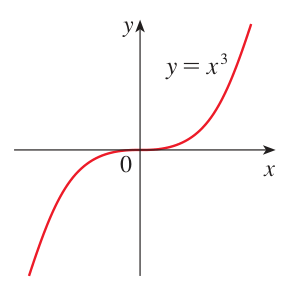
\includegraphics[width=0.92\linewidth]{images/p0318_fig1.png}
    \end{center}
    \vspace{-4pt}
    {\footnotesize\noindent\textbf{\textsf{HÌNH 12}}\quad Nếu $f(x) = x^3$, thì $f'(0) = 0$, nhưng $f$ không có cực đại hay cực tiểu.\par}

    % Khoảng cách dóng hàng để Hình 13 nằm ngang hàng với Ví dụ 6 và Cảnh báo
    \vspace{16pt}

    \begin{center}
        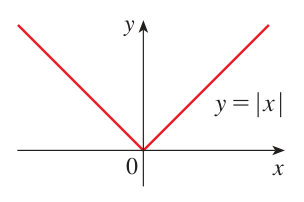
\includegraphics[width=0.92\linewidth]{images/p0318_fig2.png}
    \end{center}
    \vspace{-4pt}
    {\footnotesize\noindent\textbf{\textsf{HÌNH 13}}\quad Nếu $f(x) = |x|$, thì $f(0) = 0$ là một giá trị cực tiểu, nhưng $f'(0)$ không tồn tại.\par}
\end{minipage}%
\hfill
\begin{minipage}[t]{0.70\textwidth}
    % CỘT CHÍNH: Nội dung lý thuyết, chứng minh và các ví dụ
    \noindent Ta có thể chia cả hai vế của một bất đẳng thức cho một số dương. Do đó, nếu $h > 0$ và $h$ đủ nhỏ, ta có
    \[
    \frac{f(c + h) - f(c)}{h} \leqslant 0
    \]
    Lấy giới hạn một phía bên phải ở cả hai vế của bất đẳng thức này (sử dụng Định lý 2.3.2), ta được
    \[
    \lim_{h \to 0^+} \frac{f(c + h) - f(c)}{h} \leqslant \lim_{h \to 0^+} 0 = 0
    \]
    Nhưng vì $f'(c)$ tồn tại, nên ta có
    \[
    f'(c) = \lim_{h \to 0} \frac{f(c + h) - f(c)}{h} = \lim_{h \to 0^+} \frac{f(c + h) - f(c)}{h}
    \]
    \noindent và như vậy chúng ta đã chỉ ra rằng $f'(c) \leqslant 0$.

    Nếu $h < 0$, thì chiều của bất đẳng thức (5) bị đảo ngược khi ta chia cho $h$:
    \[
    \frac{f(c + h) - f(c)}{h} \geqslant 0
    \]
    Vì vậy, lấy giới hạn một phía bên trái, ta có
    \[
    f'(c) = \lim_{h \to 0} \frac{f(c + h) - f(c)}{h} = \lim_{h \to 0^-} \frac{f(c + h) - f(c)}{h} \geqslant 0
    \]
    Chúng ta đã chỉ ra rằng $f'(c) \geqslant 0$ và đồng thời $f'(c) \leqslant 0$. Vì cả hai bất đẳng thức này đều phải đúng, khả năng duy nhất là $f'(c) = 0$.

    Chúng ta đã chứng minh Định lý Fermat cho trường hợp cực đại địa phương. Trường hợp cực tiểu địa phương có thể được chứng minh theo cách tương tự, hoặc xem Bài tập 81 để biết một phương pháp khác.\hfill{\color{stewartred}\rule{1.15ex}{1.15ex}}

    \vspace{9pt}
    Các ví dụ sau đây nhắc nhở chúng ta không nên suy diễn quá mức từ Định lý Fermat: chúng ta không thể kỳ vọng tìm được các giá trị cực trị chỉ đơn thuần bằng cách cho $f'(x) = 0$ rồi giải tìm $x$.

    \vspace{9pt}
    \noindent\textbf{\textsf{\color{stewartcyan}VÍ DỤ 5}}\quad Nếu $f(x) = x^3$, thì $f'(x) = 3x^2$, do đó $f'(0) = 0$. Nhưng $f$ không có cực đại hay cực tiểu tại 0, như bạn có thể thấy từ đồ thị của nó ở Hình 12. (Hoặc nhận xét rằng $x^3 > 0$ khi $x > 0$ nhưng $x^3 < 0$ khi $x < 0$.) Thực tế $f'(0) = 0$ chỉ đơn giản có nghĩa là đường cong $y = x^3$ có một tiếp tuyến nằm ngang tại $(0, 0)$. Thay vì đạt cực đại hoặc cực tiểu tại $(0, 0)$, đường cong cắt ngang qua tiếp tuyến nằm ngang của nó tại điểm đó.\hfill{\color{stewartcyan}\rule{1.15ex}{1.15ex}}

    \vspace{9pt}
    \noindent\textbf{\textsf{\color{stewartcyan}VÍ DỤ 6}}\quad Hàm số $f(x) = |x|$ đạt giá trị cực tiểu (cả địa phương và tuyệt đối) tại 0, nhưng giá trị đó không thể tìm được bằng cách giải phương trình $f'(x) = 0$ bởi vì, như đã chỉ ra trong Ví dụ 2.8.5, $f'(0)$ không tồn tại. (Xem Hình 13.)\hfill{\color{stewartcyan}\rule{1.15ex}{1.15ex}}

    \vspace{9pt}
    \noindent\warningsign\hspace{0.5em}\textbf{\textsf{\color{stewartred}CẢNH BÁO}}\quad{\color{stewartred}Các Ví dụ 5 và 6 cho thấy chúng ta phải cẩn trọng khi sử dụng Định lý Fermat. Ví dụ 5 chứng minh rằng ngay cả khi $f'(c) = 0$, tại $c$ không nhất thiết phải có cực đại hay cực tiểu.} (Nói cách khác, mệnh đề đảo của Định lý Fermat nhìn chung là sai.) {\color{stewartred}Hơn nữa, một cực trị vẫn có thể tồn tại ngay cả khi $f'(c)$ không tồn tại} (như trong Ví dụ 6).

    \vspace{9pt}
    Định lý Fermat quả thực gợi ý rằng ít nhất chúng ta nên \textit{bắt đầu} tìm kiếm các giá trị cực trị của $f$ tại những số $c$ mà tại đó $f'(c) = 0$ hoặc $f'(c)$ không tồn tại. Những số như vậy được đặt cho một tên gọi đặc biệt.
\end{minipage}
